\documentclass[11pt,letterpaper]{article}
\usepackage[T1]{fontenc}
\usepackage{lmodern,microtype}
\usepackage[letterpaper,top=0.86in,bottom=0.87in,left=1.02in,right=1.02in,headheight=14pt,headsep=14pt]{geometry}
\usepackage{amsmath,amssymb,amsthm,mathtools,booktabs,array,xcolor,graphicx,fancyhdr,hyperref}
\definecolor{ink}{HTML}{19364A}
\definecolor{teal}{HTML}{12665E}
\hypersetup{colorlinks=true,urlcolor=teal,linkcolor=teal,citecolor=teal,pdftitle={Sharp parity bias for a missing Hamming ball},pdfauthor={OpenAI}}
\pagestyle{fancy}\fancyhf{}\fancyhead[L]{\small\sffamily\color{ink}Sharp parity bias for a missing Hamming ball}
\fancyhead[R]{\small\sffamily\color{ink}Quadratic characters}
\fancyfoot[C]{\small\thepage}\renewcommand{\headrulewidth}{0.3pt}
\setlength{\parindent}{0pt}\setlength{\parskip}{5pt plus 1pt minus 1pt}
\setlength{\emergencystretch}{1.7em}
\newtheoremstyle{research}{6pt}{4pt}{\itshape}{}{\bfseries\color{ink}}{.}{.5em}{}
\theoremstyle{research}
\newtheorem{theorem}{Theorem}\newtheorem{lemma}[theorem]{Lemma}
\newtheorem{corollary}[theorem]{Corollary}\newtheorem{proposition}[theorem]{Proposition}
\newcommand{\E}{\mathbb E}\newcommand{\R}{\mathbb R}\newcommand{\N}{\mathbb N}
\newcommand{\U}{U_k}\newcommand{\He}{H}
\newcommand{\rad}{\operatorname{rad}}
\newcommand{\ord}{\operatorname{ord}}
\newcommand{\low}{\mathcal B_k(a)}\newcommand{\high}{\mathcal D_k(a)}
\newcommand{\ind}{\mathbf 1}
\newcommand{\fall}[2]{(#1)_{#2}}
\newcommand{\ds}{\displaystyle}
\newcommand{\sect}[1]{\section{\texorpdfstring{\color{ink}#1}{#1}}}
\begin{document}
\thispagestyle{plain}
{\sffamily\small\color{teal} RESEARCH NOTE\hfill 26 NOVEMBER 2026}\par
{\LARGE\bfseries\color{ink} Sharp parity bias for a missing Hamming ball}\par
{\large\color{ink} Hermite thresholds and primes with prescribed quadratic signs}\par
\vspace{2pt}\hrule\vspace{4pt}
Let $q_1,\ldots,q_k\le Y$ be distinct odd primes. Given any $k$ requested Legendre
signs, how small a prime realizes more than half of them? Dirichlet GRH gives the following bounds. For every sufficiently
large $k$, a prime $p\ll k^3\log^2(2Y)$ realizes more than
$k/2+\sqrt{k}/4$ requested signs. Requiring more than $k/2+3\sqrt{k}/4$
raises our bound to $p\ll k^5\log^2(2Y)$. The reason for the different powers
lies in an extremal problem on the cube whose leading constant can be computed exactly.
\sect{The extremal problem}
For $u\in\{-1,1\}^k$ write $X(u)=k^{-1/2}\sum_i u_i$ and
$w(u)=\#\{i:u_i=-1\}$. For $A\subseteq[k]$ set $u_A=\prod_{i\in A}u_i$.
For a probability law $\mu$ its parity bias is
$\epsilon(\mu)=\max_{A\ne\varnothing}|\E_\mu u_A|$. Define
\[
 \low=\{X\le a\},\quad \high=\{X>a\},\qquad
 b_k(a)=\min_{\operatorname{supp}\mu\subseteq\low}\epsilon(\mu).
\]
Thus $b_k(a)$ is the least bias compatible with missing the open cap $\high$.
Coordinate sign changes give the same value at any center. A law of smaller bias
meets every such cap. Write $H_0=1$, $H_1=x$ and
$H_{j+1}=xH_j-jH_{j-1}$ for the monic probabilists' Hermite polynomials.
Let $h_j$ be the largest zero of $H_j$ for $j\ge1$.
\begin{theorem}[Sharp threshold]\label{th:main}
Fix $d\ge1$ and $h_d<a<h_{d+1}$. With $m=2d+1$,
\[
 \lim_{k\to\infty}k^{m/2}b_k(a)
       = C_d(a),\qquad C_d(a)=-d!\,\frac{H_{d+1}(a)}{H_d(a)}>0.
\]
At $a=h_{d+1}$, for fixed $d\ge0$, $b_k(a)\asymp_d k^{-(d+1)}$.
At $a=0$ the exact answer is $1/(k+1)$ for even $k$ and $2/(k+1)$ for odd $k$.
\end{theorem}
The interval endpoints begin at $0,1,\sqrt3,\sqrt{3+\sqrt6}$.
For $0<a<1$ the constant is $1/a-a$. For $1<a<\sqrt3$ it is
$2a(3-a^2)/(a^2-1)$. All limits hold for fixed $a$. The cube theorem is
unconditional. The prime application uses Dirichlet GRH through a smoothed
explicit formula. The lower examples establishing sharpness are probability
laws on the cube.
\begin{center}
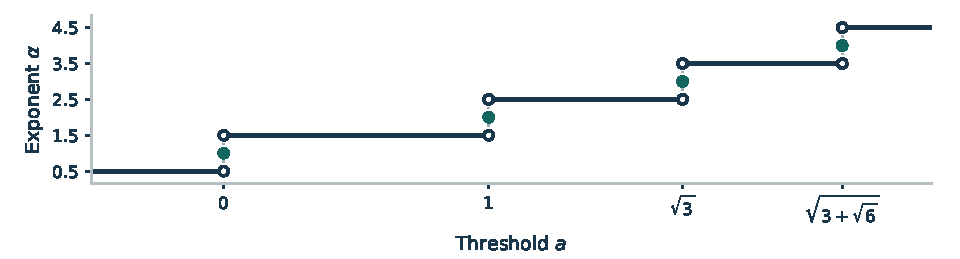
\includegraphics[width=.96\linewidth]{thresholds.pdf}\\[-3pt]
{\small The power $\alpha$ in $b_k(a)=\Theta_a(k^{-\alpha})$.
Filled dots give the exponents at the roots.}
\end{center}
\clearpage
\sect{A quadrature rule with a prescribed extreme node}
Let $G$ be standard normal. The normalized polynomials $H_j/\sqrt{j!}$
are orthonormal for $G$. This follows by integration by parts from
$H_j(x)e^{-x^2/2}=(-1)^j(d/dx)^j e^{-x^2/2}$. In this basis multiplication
by $x$ has off-diagonal entries $\sqrt j$ between positions $j-1$ and $j$,
starting at position zero. Define $J_d(c)$ to be the $(d+1)$-by-$(d+1)$
truncation to $0,\ldots,d$, with last diagonal entry changed from $0$ to $c$.
The spectral law $\nu_c$ at the first coordinate gives mass
$|\langle e_0,v\rangle|^2$ to each unit eigenvector's eigenvalue.
\begin{lemma}\label{lem:radau}
For $t>h_d$ put $c(t)=H_{d+1}(t)/H_d(t)$. The largest eigenvalue of
$J_d(c(t))$ is $t$. All its nodes are simple and their masses are positive.
The moments of $\nu_c$ through degree $2d$ agree with those of $G$.
At degree $m=2d+1$ its raw moment is $d!c$. For $d=0$ the corresponding
rule is unit mass at $t=c$.
\end{lemma}
\begin{proof}
The determinant recurrence gives characteristic polynomial
$H_{d+1}(x)-cH_d(x)$. An eigenvector is determined by its first entry since
all off-diagonals are nonzero. Thus every eigenspace has dimension one and
each mass is positive. The preceding principal block has characteristic
polynomial $H_d$. Interlacing is strict because consecutive Hermite
polynomials have no common zero by their recurrence. The eigenvalue $t>h_d$
is therefore the largest. In particular $c(t)<0$ for $h_d<t<h_{d+1}$.

A moment at $e_0$ is the sum of the weights of all walks of its length
from position zero back to zero in the tridiagonal matrix. A walk reaching
the omitted position $d+1$ needs at least $2d+2$ steps. A walk using the
changed diagonal needs at least $2d+1$. At that length its only possible
path goes directly up to $d$, stays there once, and comes directly down.
Its contribution is $d!c$. The odd Gaussian moment itself is zero.
\end{proof}
For $a$ in the open interval of Theorem~\ref{th:main}, let
$y_1,\ldots,y_d$ be the other nodes for $t=a$. Put
\[
 Q(x)=\frac{H_{d+1}(x)-c(a)H_d(x)}{x-a},\qquad
 F(x)=(x-a)Q(x)^2 .
\]
This monic polynomial has degree $m$, vanishes at every quadrature node and
is nonpositive for $x\le a$. Its lower moments cancel between the Gaussian
and the quadrature law, giving the identity
\begin{equation}\label{eq:witness}
             \E F(G)=-d!c(a)=C_d(a).
\end{equation}
For $a=1/2$, $F(x)=(x-1/2)(x+2)^2$ and $\E F(G)=3/2$.
For $a=3/2$, the witness is
$(x-3/2)(x^2+12x/5+3/5)^2$ with Gaussian mean $9/5$.
\clearpage
\sect{The Fourier lower bound and its dual meaning}
Let $\U$ be the uniform law on the cube. Write
$g(u)=\sum_A\widehat g(A)u_A$, with $\widehat g(A)=\E_{\U}[g(u)u_A]$.
Use $L(g)=\sum_A|\widehat g(A)|$ and
$L_*(g)=\sum_{A\ne\varnothing}|\widehat g(A)|$. Multiplication convolves
the coefficients, hence $L(gh)\le L(g)L(h)$ and $L(X)=\sqrt k$. Consequently
a fixed monic polynomial $F$ of degree $m$ satisfies
\begin{equation}\label{eq:cost}
 L(F(X))\le k^{m/2}+O_F(k^{(m-1)/2}).
\end{equation}
In fact the degree-$m$ terms alone have mass $(k)_m k^{-m/2}$, where
$(k)_m=k(k-1)\cdots(k-m+1)$. Each corresponding coefficient is
$m!k^{-m/2}$. Products with repeated indices from $X^m$ have total mass
$O_m(k^{m/2-1})$. These identities also describe the leading Fourier
level of the extremal witness.

For each fixed $j$, $\E_{\U}X^j=\E G^j+O_j(k^{-1})$.
Odd moments vanish. In an even moment $j=2r$, tuples consisting of $r$
distinct pairs give $(2r-1)!!(k)_r/k^r$, and all other surviving tuples
use at most $r-1$ distinct indices. Now any law on $\low$ satisfies
$\E_\mu F(X)\le0$, whereas \eqref{eq:witness} gives
$\E_{\U}F(X)=C_d(a)+O_a(k^{-1})$. Thus
\[
 C_d(a)+O_a(k^{-1})\le
 \E_{\U}F(X)-\E_\mu F(X)\le \epsilon(\mu)L_*(F(X)).
\]
With \eqref{eq:cost} this proves the lower limit in Theorem~\ref{th:main}.

There is a useful exact interpretation. For a nonempty proper subset $D$
of the cube let $\phi(D)$ denote Bella\"iche's optimized Littlewood
complexity in the abelian case \cite{bellaiche}. It is the infimum of
$L(g)/\E_{\U}g$ over real $g$ with positive mean and $g\le0$ off $D$.
\begin{proposition}\label{prop:dual}
For $D=\high$ nonempty and proper, $\phi(D)=1+1/b_k(a)$.
\end{proposition}
\begin{proof}
Let $v(u)=(u_A)_{A\ne\varnothing}$. The definition of $b_k(a)$ is the
distance in $\ell^\infty$ of $0$ from the convex hull of the $v(u)$
with $u\in\low$. Finite-dimensional minimax gives
$b_k(a)=\max_{\|z\|_1\le1}\min_{u\in\low}z\cdot v(u)$.
It is positive since a law with all nonconstant Fourier coefficients zero
is uniform. An optimizing $z$ gives $g=b_k(a)-z\cdot v$.
Conversely, if $g$ has mean $c>0$ and nonconstant coefficients $s$,
then $-s\cdot v\ge c$ off $D$. The minimax identity gives
$c\le b_k(a)\|s\|_1$. These two inequalities prove the formula.
\end{proof}
This identifies the sharp asymptotic cost among \emph{all} real functions
detecting the cap. The degree-$m$ polynomial already attains it to first order.
\clearpage
\sect{Matching laws on both parities of Hamming layers}
Fix $h_d<t_1<t_2<a$. Mix the two spectral laws with endpoints $t_1,t_2$
in equal proportions. Their combined $2d+2=m+1$ nodes are distinct.
Indeed their characteristic polynomials differ by a nonzero multiple of
$H_d$. Equal values of $c$ would give equal largest nodes, and consecutive
Hermite polynomials have no common zero. Each mass is positive. Through degree
$m-1$ the mixed moments are Gaussian, and the last moment is
\[
                 M=\frac{d!}{2}\big(c(t_1)+c(t_2)\big).
\]
Round every node to the nearest attainable value of $X$ on layers of even
$w$. Round a second copy on layers of odd $w$. Each mesh is $4/\sqrt k$.
For sufficiently large $k$, the nodes within each list stay distinct and
strictly below $a$. On each list solve for the $m+1$ weights whose moments are
\begin{equation}\label{eq:momenttarget}
       \E_{\U}X^j\quad(0\le j<m),\qquad M\quad(j=m).
\end{equation}
Both Vandermonde matrices converge to the same invertible matrix. Both
solutions converge to the strictly positive original weights, so each is
a probability distribution. Choose each parity with probability $1/2$,
choose a layer by its fitted weights, and sample uniformly within it.
This constructs a law $\mu_k$ on at most $4d+4$ layers.

Let $R_j(w)$ denote the expectation of a product of $j$ distinct coordinates
on a uniform layer of weight $w$. With $s=k-2w=\sqrt k\,X$,
\begin{equation}\label{eq:K}
 \sum_{j=0}^k\binom{k}{j}R_j(w)z^j=(1-z)^w(1+z)^{k-w},\qquad
 R_{k-j}(w)=(-1)^w R_j(w).
\end{equation}
Multiplication by the coordinate sum gives
$s R_j=jR_{j-1}+(k-j)R_{j+1}$, starting with $R_0=1$ and $R_1=s/k$.
It follows that $(k)_jR_j$ is monic of degree $j$ in $s$. Hence on each parity
the expected level-$j$ bias is zero for $1\le j<m$, and at $j=m$ it is exactly
$M k^{m/2}/(k)_m$. Indeed the lower moments agree with the uniform cube
and its $m$th moment is zero. The two parity fits have identical moments
through $m$. The complementary levels $k-m,\ldots,k$ therefore vanish in the mixture.

To bound the middle levels let $\pi_w=2^{-k}\binom{k}{w}$. Orthogonality
of the Walsh characters gives
$\sum_w\pi_w R_j(w)^2=1/\binom{k}{j}$ by expanding the squared average of
all $\binom{k}{j}$ characters. For the chosen layers, $|X|$ is bounded,
hence $\pi_w\gg_{t_1,t_2,d}k^{-1/2}$ by Stirling's formula. Uniformly for
$m+1\le j\le k-m-1$ we obtain
\[
 |R_j(w)|\ll \frac{k^{1/4}}{\sqrt{\binom{k}{m+1}}}
                =O(k^{-m/2-1/4}).
\]
Thus $\limsup k^{m/2}b_k(a)\le |M|$. Sending both endpoints up to $a$
gives $|M|\to C_d(a)$, completing the open-interval proof.
\clearpage
\sect{Rigidity of near minimizers}
The same polynomial determines which layers carry mass in an asymptotically
optimal construction. It also identifies which coordinate tests must show bias.
\begin{theorem}\label{th:rigid}
Let $h_d<a<h_{d+1}$, $m=2d+1$ and $C=C_d(a)$. Suppose
$\operatorname{supp}\mu_k\subseteq\low$ and
$k^{m/2}\epsilon(\mu_k)\le C+o(1)$. Under $\mu_k$, the law of $X$ converges
weakly to the spectral law $\nu_{c(a)}$. Moreover
\begin{equation}\label{eq:rigid}
 \frac1{\binom{k}{m}}\sum_{|A|=m}
  \left|k^{m/2}\E_{\mu_k}u_A+C\right|\longrightarrow0.
\end{equation}
No coordinate symmetry is required of the laws.
\end{theorem}
\begin{proof}
We have $0\le\E_{\mu_k}[-F(X)]\le
\epsilon(\mu_k)L_*(F(X))-\E_{\U}F(X)=o(1)$, with the last upper
bound following from \eqref{eq:witness} and \eqref{eq:cost}.
On $(-\infty,a]$, the nonnegative function $-F$ vanishes precisely at the
$d+1$ nodes of $\nu_{c(a)}$ and grows like $|x|^m$ at the negative end.
It has positive infimum outside any fixed neighborhood of those nodes.
Thus the mass outside the neighborhood tends to zero, the laws are tight,
and their absolute moments of order $m$ are bounded. For $j<m$,
\[
 \bigl|\E_{\mu_k}X^j-\E_{\U}X^j\bigr|
 \le \epsilon(\mu_k)k^{j/2}=o(1).
\]
Uniform integrability at every order below $m$ lets these moments pass
to subsequential limits. Any such limit lies on the stated nodes. Its
moments of orders $0,\ldots,d$ uniquely recover the node weights by a
Vandermonde system. Lemma~\ref{lem:radau} supplies those weights.

In $F(X)$ the Fourier mass below degree $m$, except for the constant,
is $O_F(k^{(m-1)/2})$, by the expansion leading to \eqref{eq:cost}.
Its contribution to the bias is $o(1)$. The top coefficients are all
$m! k^{-m/2}$. Since $\E_{\mu_k} F(X)-\E_{\U}F(X)\to-C$, the
average over $|A|=m$ of $k^{m/2}\E_{\mu_k}u_A$ tends to $-C$.
Every summand is bounded below by $-C-o(1)$ uniformly in $A$.
This proves \eqref{eq:rigid}.
\end{proof}
\textbf{The first interval in explicit terms.}
For $0<a<1$ the limiting law puts mass $1/(1+a^2)$ at $a$ and mass
$a^2/(1+a^2)$ at $-1/a$. The two masses make its mean zero and its variance
one. Its third moment is $a-1/a$. At $a=1/2$, four fifths of the limiting
mass lies at $1/2$ and one fifth at $-2$. The mean signed three-coordinate
bias, multiplied by $k^{3/2}$, tends to $-3/2$. These conclusions hold
even if the original measures assign different weights to individual words
in the same layer.
\clearpage
\sect{The transition values}
\label{sec:endpoint}

At a Hermite zero the optimal exponent lies halfway between the exponents on
the two neighboring open intervals. For each fixed $d\geq 0$, with $a=h_{d+1}$,
we have
\begin{equation}
  b_k(a)=\Theta_d(k^{-d-1}).                                      \label{eq:endpoint}
\end{equation}
This includes $a=h_1=0$. We give the details because the support condition
at equality makes direct rounding of a Gaussian quadrature rule delicate.

\paragraph{Lower bound.}
Put $q(x)=H_{d+1}(x)/(x-a)$ and $F_k(x)=(x+\sqrt{k})(x-a)q(x)^2$.
On the permitted part of the cube $-\sqrt{k}\le x\le a$, we have $F_k(x)\le0$.
Write $Z$ for a standard Gaussian. Orthogonality to $q$ gives
$\mathbb E[(Z-a)q(Z)^2]=0$, and consequently
\[
  \mathbb E[Z(Z-a)q(Z)^2]=\mathbb E[H_{d+1}(Z)^2]=(d+1)!.
\]
For every fixed polynomial the uniform-cube expectation at $X$ equals its
Gaussian expectation up to $O_d(k^{-1})$ (with constants depending on that
polynomial). Indeed the moments of odd order vanish, and in each even moment
the pairings of distinct indices give the Gaussian main term with error
$O_d(k^{-1})$. Hence $\mathbb E_{\rm unif}F_k(X)=(d+1)!+O_d(k^{-1/2})$.
The sum of the absolute Walsh coefficients of $X^j$ is at most $k^{j/2}$,
by expanding the $j$-fold product. It follows term by term that the sum for
$F_k(X)$ is $O_d(k^{d+1})$. Comparing the uniform expectation with the
expectation for any supported law proves the lower bound in
\eqref{eq:endpoint}.

\paragraph{An interior quadrature rule.}
Let $m=d+1$ and write $z_1<\cdots<z_m=a$ for the zeros of $H_m$.
Let $J(t)$ be the $m$-by-$m$ tridiagonal Hermite matrix with off-diagonal
entries $\sqrt{1},\ldots,\sqrt{m-1}$ and diagonal entries zero except for
the last, which is $t$. Its spectral distribution at the first coordinate
has positive weights at its $m$ simple eigenvalues $z_i(t)$. The eigenvector
recurrence shows that both endpoint coordinates are nonzero, and
$z_i'(0)$ is the square of the last coordinate of a normalized eigenvector.
In particular $z_i'(0)>0$. Spectral weights are continuous near $0$.
Every one of these distributions integrates the Gaussian moments of orders
$0$ through $2d$. Indeed the moments are $(J(t)^j)_{11}$, and a walk from
the first coordinate using the final diagonal entry and returning needs
at least $2d+1$ steps. The rule at $t=0$ is Gaussian quadrature.

Choose a constant $L>12/z_m'(0)$ and take $t=-L/\sqrt{k}$.
For all sufficiently large $k$, even the largest node satisfies
$z_m(t)<a-10/\sqrt{k}$. Each node is within $L/\sqrt{k}$ of its
corresponding zero $z_i$, by the operator norm bound on $J(t)-J(0)$.
The nodes remain separated, and their weights stay bounded below by a
positive constant depending on $d$.

\clearpage
\paragraph{Exact moment matching after rounding.}
Write $w$ for the number of minus signs, so $X=(k-2w)/\sqrt{k}$.
Fix one of the two parities of $w$. For each node choose two attainable
values of $X$ of this parity, one on either side at distance between
$4/\sqrt{k}$ and $8/\sqrt{k}$. This is possible because the mesh is
$4/\sqrt{k}$, and all these values still lie below $a$. Split each
original weight between its two neighbors by linear interpolation,
preserving the original node's mean. Both fractions are at least $1/3$.
For every fixed monomial of degree at most $2d+1$, Taylor's theorem on a
fixed compact interval gives a total interpolation error $O_d(k^{-1})$.

At the $2m=2d+2$ grid nodes prescribe the exact uniform-cube moments through
$2d$, and prescribe the original $J(t)$ moment for degree $2d+1$. The
split weights miss each of these targets by $O_d(k^{-1})$. Through $2d$
the original rule has the Gaussian moments, whose discrepancies from the
cube moments are $O_d(k^{-1})$. Correct all the weights by solving the
square Vandermonde system for these errors. The inverse has entries
$O_d(\sqrt{k})$. Indeed the coefficients of the Lagrange basis polynomials
have this bound, since each denominator has one factor of order
$k^{-1/2}$ and all the other factors stay bounded away from zero, while the
numerator coefficients stay bounded. Thus each weight changes by
$O_d(k^{-1/2})$ and remains positive. The zeroth moment keeps their sum one.
Carry out this construction on each parity, spread each mass uniformly over
its layer, and average the two probability laws. In each parity the moments
through $2d$ match the cube exactly, and all the supporting values lie
within $O_d(k^{-1/2})$ of a zero of $H_{d+1}$.

\paragraph{Bias on every level.}
Let $K_j(w)$ be the sum of the Walsh characters of size $j$ on the layer
$w$. Then $P_{j,k}(x)=j!k^{-j/2}K_j(w)$ is monic in $x=X$. For fixed $j$
it stays bounded on compact intervals, as follows from $P_{0,k}=1$,
$P_{1,k}=x$, and
\[
 P_{j+1,k}=xP_{j,k}-j\bigl(1-(j-1)/k\bigr)P_{j-1,k}.
\]
For $1\le j\le 2d$ its expectation on each parity is zero by exact moment
matching. For $j=2d+1$, the polynomial $P_{j,k}-H_{d+1}H_d$ has degree at
most $2d$ and uniform-cube mean zero by oddness. On the supporting layers
$H_{d+1}H_d=O_d(k^{-1/2})$. Thus the expectation of $P_{2d+1,k}$ on each
parity is $O_d(k^{-1/2})$. Dividing the expected $K_j$ by $\binom{k}{j}$
gives the bias of each character of that size. The bound for $j=2d+1$ is
therefore $O_d(k^{-d-1})$, and the same bound holds pointwise on the
support for $j=2d+2$ by the fixed-degree recurrence. Reflection
$K_{k-j}(w)=(-1)^wK_j(w)$ controls the corresponding upper levels, with
the top level zero by equal parity masses.

For $2d+3\le j\le k-2d-3$, orthogonality of the layer characters gives
\[
 \frac{|K_j(w)|}{\binom{k}{j}}
  \le \left(\frac{2^k}{\binom{k}{w}\binom{k}{j}}\right)^{1/2}
  = O_d(k^{-d-5/4}).
\]
Here $|k-2w|=O_d(\sqrt{k})$, so $2^k/\binom{k}{w}=O_d(\sqrt{k})$ by
Stirling's formula. This proves the upper bound in \eqref{eq:endpoint}.

\clearpage
\sect{Exact finite answer up to the equator}
There is an exact formula on the other side of the first Hermite threshold.
It explains the even--odd difference at $a=0$.
\begin{proposition}\label{prop:majority}
Let $-k\le s\le0$ be an integer congruent to $k$ modulo $2$. The minimum
bias of a law supported on $\sum u_i\le s$ is $(1-s)/(k+1)$.
\end{proposition}
\begin{proof}
Write $S=\sum_i u_i$ and let $w_0=(k-s)/2$ be the top allowed layer.
For every allowed word,
$S\le s-1+(-1)^{w-w_0}$. If the bias is $\epsilon$, taking expectations
gives $-k\epsilon\le\E S\le s-1+\epsilon$, proving the lower bound.

For the upper bound set $N=k+1$, $t=1-s$. Choose a uniform word on
the $N$-cube with coordinate sum $-t$ and discard its last coordinate.
Its remaining sum lies in $\{s,s-2\}$. On any such slice with
$t\ge1$, the absolute moment of a product of $j$ coordinates is at most
$t/N$ for $1\le j\le N-1$. We give the slice argument, also known as
a Krawtchouk eigenvalue bound \cite{kraw}.

Write $r_j$ for the signed moment. At $j=1$ the claim follows by averaging
the coordinate sum, and at $j=N-1$ it follows by complementation.
For $t\ge2$, distinguish a fixed negative sign in the population and draw
a uniform $j$-subset. Conditional on including or omitting that sign, the
remaining sample is uniform in a population of size $N-1$ and imbalance
$t-1$. For $2\le j\le N-2$ both remaining degrees lie between $1$ and $N-2$.
Induction on $t$ bounds $|r_j|$ by $(t-1)/(N-1)\le t/N$.

At $t=1$, $N=2l+1$. The generating polynomial in \eqref{eq:K} is
$(1-z)(1-z^2)^l$. Complementation reduces the check to even degrees
$2i$, $1\le i\le l$. Then
$|r_{2i}|=\binom{l}{i}/\binom{2l+1}{2i}$. The reciprocal equals $N$
at $i=1,l$, and the ratio of consecutive reciprocals is
$(2l-2i+1)/(2i+1)$, decreasing with $i$. Hence the reciprocal has its
minimum at an endpoint. This proves the slice bound and the proposition.
\end{proof}
Taking $s=0$ for even $k$ and $s=-1$ for odd $k$ gives the strict-majority
values of Theorem~\ref{th:main}. For fixed $a<0$, taking the largest attainable
$s\le a\sqrt k$ gives $b_k(a)=|a|/\sqrt k+O_a(1/k)$.

\textbf{Dependence on the threshold.}
Between two consecutive roots the leading constant tends to zero as $a$
approaches the upper root and diverges as $a$ approaches the lower root.
The one-sided value of $C_d(a)$ cannot be substituted at a root. Even the
first root has two different constants along the two parity subsequences.
\clearpage
\sect{Primes realizing a prescribed fraction of quadratic signs}
Let $q_1,\ldots,q_k$ be distinct odd primes at most $Y$.
For a sign word $v$ and a prime $p\nmid \prod_i q_i$, define
$M_v(p)=\#\{i:(\frac{p}{q_i})=v_i\}$. Define $D(a)$ for fixed $a\ge0$ by
\[
 D(a)=
 \begin{cases}2d+1,& h_d<a<h_{d+1},\quad d\ge1,\\
               2d+2,& a=h_{d+1},\quad d\ge0 .
 \end{cases}
\]
\begin{theorem}\label{th:prime}
For every sufficiently large $k$ depending on $a$, and every $v\in\{-1,1\}^k$,
there is a prime $p\nmid\prod_i q_i$ such that
\[
 M_v(p)>\frac{k+a\sqrt k}{2},\qquad
 p\ll_a k^{D(a)}\log^2(2Y).
\]
The bound is uniform in the primes and in $v$.
\end{theorem}
\begin{proof}
Put $D=D(a)$ and $Q=\prod_i q_i$. Use the witness $F(X)$ of
\eqref{eq:witness} in an open interval and $F_k(X)$ of
Section~\ref{sec:endpoint} at a root. Translate the witness by $u_i\mapsto
v_i u_i$ and call it $g$. Translation preserves the uniform mean and the
absolute values of all coefficients. In both cases $g$ has positive mean
$g_0\gg_a 1$, $L(g)\ll_a k^{D/2}$, and degree at most $D$.
A positive value forces the required strict inequality for $M_v$.

For $A\subseteq[k]$ the product character $\chi_A=\prod_{i\in A}
(\frac{\cdot}{q_i})$ is primitive of conductor $f_A=\prod_{i\in A}q_i$.
The empty product has conductor $1$. This follows from the Chinese
remainder theorem and the primitivity of each Legendre symbol. For
$|A|\le D$ we have $\log(2f_A)\le D\log(2Y)$. The once-smoothed Dirichlet
explicit formula gives, for $x\ge3$,
\begin{equation}\label{eq:primeestimate}
\sum_{p<x,\,p\nmid Q}(1-p/x)\log p\,\chi_A(p)
 =\ind_{A=\varnothing}\frac x2+
 O\!\left(\sqrt x\log(2f_A)+\log\rad Q\right).
\end{equation}
Apply the degree-one proof of Bella\"iche's Lemma 6
\cite{bellaiche} to $-L'/L$ with kernel $x^{s}/(s(s+1))$.
The pole of $-\zeta'/\zeta$ has residue $1$, giving $x/2$.
Dirichlet GRH bounds the zero sum by $O(\sqrt x\log(2f_A))$ as in that
lemma. Higher prime powers contribute $O(\sqrt x)$ since
$\sum_{j\ge2,\,2^j\le x}\vartheta(x^{1/j})\ll\sqrt x+x^{1/3}\log(2x)\ll\sqrt x$,
by Chebyshev's bound. Removing primes dividing $Q$ costs
at most $\log\rad Q$.
Multiply \eqref{eq:primeestimate} by $\widehat g(A)$ and sum. The result is
\[
  \tfrac12xg_0+O_a\!\left(k^{D/2}
       [\sqrt x\log(2Y)+k\log(2Y)]\right).
\]
Take $x=K_a k^D\log^2(2Y)$ with $K_a$ sufficiently large. Since $D\ge2$,
the main term dominates both errors. A positive smoothed sum has a prime
with $g>0$.
\end{proof}
\clearpage
\sect{Finite checks and the scope of the sharpness result}
The arithmetic argument needs only the characters occurring in the witness.
More generally, take primitive quadratic characters of conductors $f_i$, and
exclude all primes dividing a multiple $Q$ of their conductors. If every
nonempty product of at most $D$ characters is nonprincipal, the same proof
applies. The product conductor divides $\prod_{i\in A}f_i$.
With $Y=\max_i f_i$, the resulting prime bound is
\[
 p\ll_a k^D\log^2(2Y)+k^{D/2}\log\rad Q.
\]
Relations among more than $D$ of the chosen characters are permitted.
For any particular witness one may also sum the conductor errors in
\eqref{eq:primeestimate} using the individual $|\widehat g(A)|$.

\textbf{Finite example.} Use the twelve odd primes $3$ through $41$.
There are $4{,}096$ possible target sign words. For each prime cutoff,
the checker computes, for every target, the distance to its closest
available prime word. The worst such distance first falls to $5$ at $79$,
to $4$ at $229$, and to $3$ at $691$. The exact cutoffs for guaranteeing
at least seven and at least nine matching signs are $79$ and $691$, respectively. Both cutoffs include the prime at the endpoint.

\begin{center}\small
\begin{tabular}{@{}rrr@{\qquad}l@{}}
\toprule
$k$ & $a$ & maximum distance in $\high$ & exact $b_k(a)$\\
\midrule
8 & $1/2$ & $3$ & $1/9$\\
8 & $3/2$ & $1$ & $1/69$\\
12 & $1/2$ & $5$ & $1/13$\\
12 & $3/2$ & $3$ & $1/104$\\
17 & $1/2$ & $7$ & $1/33$\\
17 & $3/2$ & $5$ & $53/13717$\\
\bottomrule
\end{tabular}
\end{center}
The finite values are verified by rational primal and dual certificates.
A second script constructs eight-layer laws and bounds every Fourier
level at five dimensions. At $k=10^{16}$ it gives the outward-rounded bracket
\[
  1.49999994 < k^{3/2}b_k(1/2) < 1.50100041 .
\]
The largest bias of the constructed law is attained at degree three.

The exact asymptotic in Theorem~\ref{th:main} controls what can be deduced
from a uniform bound on individual parity biases. A lower bound on the
least prime for a worst-case choice of moduli would require an arithmetic
construction. Theorem~\ref{th:prime} supplies upper bounds. Its constants
are left unevaluated.

\textbf{Further research questions.}
What are the subsequential leading constants at $h_2,h_3,\ldots$? How does
the minimum bias change when $a$ approaches one of these roots at rate
$k^{-1/2}$? Can correlations among the prime character sums improve the
powers of $k$ in Theorem~\ref{th:prime}?
\clearpage
\sect{Sources and relation to earlier work}
The readable edition of \texttt{lsernau/grh-lean} exposes Mathlib's
\texttt{RiemannHypothesis} and the Dirichlet theorems
\texttt{LFunction\_ne\_zero\_of\_half\_lt\_re} and
\texttt{LFunction\_eq\_zero\_re}. The first Dirichlet statement excludes
zeros in $\Re s>1/2$ with the principal pole excepted. The second puts
all zeros in $0<\Re s<1$ on the line. Its guide traces a one-sided
smoothed prime bound to the zero theorem. Our prime application runs
from the Dirichlet zero theorem through the explicit formula to a positive
one-sided test. We inspected the pinned Lean source and the project's
reports of its build and axiom checks. This note gives human-readable
proofs of the new statements. The upstream build was not rerun here.
The Lean FRO and Mathlib Initiative describe their independent checks
of Alpöge's original RH proof \cite{lean,fro}. The requested Wikipedia
article supplies background on the critical line and explicit formula
\cite{wiki}.

The ProveIt index describes 61 filed reports and states how they were
archived. Its reports on symmetric-power character polynomials and
one-sided prime tests motivate optimizing the sign and Fourier cost of
a witness \cite{proveit}. A review of the filed README files and the
descriptions in 42 further incoming archives, together with targeted
literature searches, found no statement of the open-interval Hermite-ratio
formula. This is the extent of the priority check.

Bellaïche's least-prime theorem already optimizes over one-sided
class functions. Bazzi and Nahas use the dual small-bias problem for
read-once formulas. Bazzi treats the covering radius under exact limited
independence. Derksen, Ivanov, Lee and Viola construct small-bias
distributions on few central layers, including their Theorem 6 on
two-sided concentration. Hanson, Vaughan and Zhang study prescribed
Legendre symbols of integers. The result here computes an exact
one-sided constant, identifies its near minimizers, and applies a
low-degree witness to prime sign patterns \cite{bellaiche,cnf,bazzi,dilv,hvz}.

\begingroup\small
\begin{thebibliography}{10}\setlength{\itemsep}{0pt}\setlength{\parskip}{0pt}
\bibitem{lean} \texttt{lsernau/grh-lean}, \href{https://github.com/lsernau/grh-lean/tree/72fead102f663d5c7a407964a13dc0cf9d977207}{\emph{GRH for Dirichlet $L$-functions, in Lean 4}}, revision \texttt{72fead1}.
\bibitem{fro} Lean FRO and Mathlib Initiative, \href{https://leanprover-community.github.io/blog/posts/riemann-hypothesis/}{\emph{Lean verification of the Riemann Hypothesis}}, 21 November 2026.
\bibitem{wiki} Wikipedia, \href{https://en.wikipedia.org/wiki/Riemann_hypothesis}{\emph{Riemann hypothesis}}, consulted 26 November 2026.
\bibitem{proveit} V. Reshetnikov, \href{https://github.com/VladimirReshetnikov/ProveIt/tree/2c45d198070f93209d6f0faa2d387ef0a2c4e72c/Analysis/GeneralizedRiemannHypothesis}{\emph{ProveIt, Generalized Riemann Hypothesis collection}}, revision \texttt{2c45d19}.
\bibitem{bellaiche} J. Bellaïche, \href{https://doi.org/10.24033/asens.2291}{Théorème de Chebotarev et complexité de Littlewood}, \emph{Ann. Sci. Éc. Norm. Supér.} \textbf{49} (2016), 579--632, esp.\ pp.\ 608--610.
\bibitem{cnf} L. Bazzi and N. Nahas, \href{https://eccc.weizmann.ac.il/report/2013/034/}{Small-bias is not enough to hit read-once CNF}, ECCC TR13-034 (2013).
\bibitem{bazzi} L. Bazzi, \href{https://arxiv.org/abs/1707.00552}{On the tightness of Tietäväinen's bound for distributions with limited independence}, arXiv:1707.00552.
\bibitem{dilv} H. Derksen, P. Ivanov, C. H. Lee and E. Viola, \href{https://eccc.weizmann.ac.il/report/2025/021/}{Pseudorandomness, symmetry, smoothing: II}, ECCC TR25-021.
\bibitem{hvz} B. Hanson, R. C. Vaughan and R. Zhang, \href{https://arxiv.org/abs/1605.05584}{The least number with prescribed Legendre symbols}, arXiv:1605.05584.
\bibitem{kraw} A. E. Brouwer, S. M. Cioabă, F. Ihringer and M. McGinnis, \href{https://arxiv.org/abs/1709.09011}{The smallest eigenvalues of Hamming graphs, Johnson graphs and other distance-regular graphs with classical parameters}, Theorem 1.2(i).
\end{thebibliography}
\endgroup
\end{document}
